%%%%%%%%%%%%%%%%%%%%%%%%%%%%%%%%%%%%%%%%%
% Arsclassica Article
% LaTeX Template
% Version 1.1 (10/6/14)
%
% This template has been downloaded from:
% http://www.LaTeXTemplates.com
%
% Original author:
% Lorenzo Pantieri (http://www.lorenzopantieri.net) with extensive modifications by:
% Vel (vel@latextemplates.com)
% Johan Bos (johan.bos@rug.nl)
% Barbara Plank (bapl@itu.dk)
% 
% License:
% CC BY-NC-SA 3.0 (http://creativecommons.org/licenses/by-nc-sa/3.0/)
%
%%%%%%%%%%%%%%%%%%%%%%%%%%%%%%%%%%%%%%%%%

%----------------------------------------------------------------------------------------
%	PACKAGES AND OTHER DOCUMENT CONFIGURATIONS
%----------------------------------------------------------------------------------------

\documentclass[
10pt, % Main document font size
a4paper, % Paper type
oneside, % One page layout (no page indentation)
headinclude,footinclude, % Extra spacing for the header and footer
%BCOR5mm, % Binding correction
] {book}%
\usepackage{eurosym}
\usepackage{booktabs} % for nice tables with \toprule, \midrule
\usepackage{csvsimple,longtable}
\setcounter{secnumdepth}{5}
%%%%%%%%%%%%%%%%%%%%%%%%%%%%%%%%%%%%%%%%%
% Wenneker Article
% Structure Specification File
% Version 1.0 (28/2/17)
%
% This file originates from:
% http://www.LaTeXTemplates.com
%
% Authors:
% Frits Wenneker
% Vel (vel@LaTeXTemplates.com)
%
% License:
% CC BY-NC-SA 3.0 (http://creativecommons.org/licenses/by-nc-sa/3.0/)
%
%%%%%%%%%%%%%%%%%%%%%%%%%%%%%%%%%%%%%%%%%

%----------------------------------------------------------------------------------------
%	PACKAGES AND OTHER DOCUMENT CONFIGURATIONS
%----------------------------------------------------------------------------------------

\usepackage[english]{babel} % English language hyphenation

\usepackage{microtype} % Better typography

\usepackage{amsmath,amsfonts,amsthm} % Math packages for equations

\usepackage[svgnames]{xcolor} % Enabling colors by their 'svgnames'

\usepackage[hang, small, labelfont=bf, up, textfont=it]{caption} % Custom captions under/above tables and figures

\usepackage{booktabs} % Horizontal rules in tables

\usepackage{lastpage} % Used to determine the number of pages in the document (for "Page X of Total")

\usepackage{graphicx} % Required for adding images

\usepackage{enumitem} % Required for customising lists
\setlist{noitemsep} % Remove spacing between bullet/numbered list elements

\usepackage{sectsty} % Enables custom section titles
\allsectionsfont{\usefont{OT1}{phv}{b}{n}} % Change the font of all section commands (Helvetica)

\usepackage[hidelinks,
			colorlinks=true,
			linkcolor=black,
			citecolor=blue,
			urlcolor=blue]{hyperref}

\usepackage{graphicx}
\graphicspath{ {./img/} }

\usepackage{xcolor}

\usepackage[toc,page]{appendix}

%----------------------------------------------------------------------------------------
%	MARGINS AND SPACING
%----------------------------------------------------------------------------------------

\usepackage{geometry} % Required for adjusting page dimensions

\geometry{
	top=1cm, % Top margin
	bottom=1.5cm, % Bottom margin
	left=2cm, % Left margin
	right=2cm, % Right margin
	includehead, % Include space for a header
	includefoot, % Include space for a footer
	%showframe, % Uncomment to show how the type block is set on the page
}

\setlength{\columnsep}{7mm} % Column separation width

\setlength\parindent{0pt} % No intent on new paragraphs

\renewcommand{\baselinestretch}{1.2} % Line spacing

%----------------------------------------------------------------------------------------
%	FONTS
%----------------------------------------------------------------------------------------

\usepackage[T1]{fontenc} % Output font encoding for international characters
\usepackage[utf8]{inputenc} % Required for inputting international characters

\usepackage{XCharter} % Use the XCharter font

%----------------------------------------------------------------------------------------
%	HEADERS AND FOOTERS
%----------------------------------------------------------------------------------------

\usepackage{fancyhdr} % Needed to define custom headers/footers
\pagestyle{fancy} % Enables the custom headers/footers

\renewcommand{\headrulewidth}{0.0pt} % No header rule
\renewcommand{\footrulewidth}{0.0pt} % Thin footer rule

\renewcommand{\sectionmark}[1]{\markboth{#1}{}} % Removes the section number from the header when \leftmark is used

%\nouppercase\leftmark % Add this to one of the lines below if you want a section title in the header/footer

% Headers
\lhead{} % Left header
% \chead{\textit{\thetitle}} % Center header - currently printing the article title
\rhead{} % Right header

% Footers
\lfoot{} % Left footer
\cfoot{} % Center footer
\rfoot{\footnotesize Page \thepage\ of \pageref{LastPage}} % Right footer, "Page 1 of 2"

\fancypagestyle{firstpage}{ % Page style for the first page with the title
	\fancyhf{}
	\renewcommand{\footrulewidth}{0pt} % Suppress footer rule
}

%----------------------------------------------------------------------------------------
%	TITLE SECTION
%----------------------------------------------------------------------------------------

\newcommand{\authorstyle}[1]{{\large\usefont{OT1}{phv}{b}{n}\color{Black}#1}} % Authors style (Helvetica)

\newcommand{\institution}[1]{{\footnotesize\usefont{OT1}{phv}{m}{sl}\color{Black}#1}} % Institutions style (Helvetica)

\usepackage{titling} % Allows custom title configuration

\newcommand{\HorRule}{\color{Gray}\rule{\linewidth}{1pt}} % Defines the gold horizontal rule around the title

\pretitle{
	\vspace{-30pt} % Move the entire title section up
	\HorRule\vspace{10pt} % Horizontal rule before the title
	\fontsize{22}{26}\usefont{OT1}{phv}{b}{n}\selectfont % Helvetica
	\color{DarkRed} % Text colour for the title and author(s)
}

\posttitle{\par\vskip 15pt} % Whitespace under the title

\preauthor{} % Anything that will appear before \author is printed

\postauthor{ % Anything that will appear after \author is printed
	\vspace{10pt} % Space before the rule
	\par\HorRule % Horizontal rule after the title
	\vspace{20pt} % Space after the title section
}

%----------------------------------------------------------------------------------------
%	ABSTRACT
%----------------------------------------------------------------------------------------

\usepackage{lettrine} % Package to accentuate the first letter of the text (lettrine)
\usepackage{fix-cm}	% Fixes the height of the lettrine

\newcommand{\initial}[1]{ % Defines the command and style for the lettrine
	\lettrine[lines=3,findent=4pt,nindent=0pt]{% Lettrine takes up 3 lines, the text to the right of it is indented 4pt and further indenting of lines 2+ is stopped
		\color{DarkGoldenrod}% Lettrine colour
		{#1}% The letter
	}{}%
}

\usepackage{xstring} % Required for string manipulation

\newcommand{\lettrineabstract}[1]{
	\StrLeft{#1}{1}[\firstletter] % Capture the first letter of the abstract for the lettrine
	\initial{\firstletter}\textbf{\StrGobbleLeft{#1}{1}} % Print the abstract with the first letter as a lettrine and the rest in bold
}

%----------------------------------------------------------------------------------------
%	BIBLIOGRAPHY
%----------------------------------------------------------------------------------------

\usepackage[backend=bibtex,style=authoryear,natbib=true]{biblatex} % Use the bibtex backend with the authoryear citation style (which resembles APA)

\addbibresource{example.bib} % The filename of the bibliography

\usepackage[autostyle=true]{csquotes} % Required to generate language-dependent quotes in the bibliography

\setlength\bibitemsep{4.0\itemsep}
 % Include the structure.tex file which specified the document structure and layout


%----------------------------------------------------------------------------------------
%	HYPHENATION
%----------------------------------------------------------------------------------------

\hyphenation{Fortran hy-phen-ation} % Specify custom hyphenation points in words with dashes where you would like hyphenation to occur, or alternatively, don't put any dashes in a word to stop hyphenation altogether



%----------------------------------------------------------------------------------------
%	TITLE AND AUTHOR(S)
%----------------------------------------------------------------------------------------

\title{\normalfont\spacedallcaps{title}} % The article title

\author{\spacedlowsmallcaps{author}} % The article author(s) - author affiliations need to be specified in the AUTHOR AFFILIATIONS block

\date{\today} % An optional date to appear under the author(s)

%----------------------------------------------------------------------------------------

\begin{document}

%----------------------------------------------------------------------------------------
%	HEADERS
%----------------------------------------------------------------------------------------

%\renewcommand{\chaptermark}[1]{\markright{\spacedlowsmallcaps{#1}}} % The header for all pages (oneside) or for even pages (twoside)
%\renewcommand{\subsectionmark}[1]{\markright{\thesubsection~#1}} % Uncomment when using the twoside option - this modifies the header on odd pages
%\lehead{\mbox{\llap{\small\thepage\kern1em\color{halfgray} \vline}\color{halfgray}\hspace{0.5em}\rightmark\hfil}} % The header style

\pagestyle{scrheadings} % Enable the headers specified in this block


%----------------------------------------------------------------------------------------
%	TITLE PAGE
%----------------------------------------------------------------------------------------

\hypersetup{pageanchor=false}
\begin{titlepage}
\thispagestyle{empty}
\begin{figure}[h!] %  figure placement: here, top, bottom, or page
\centering

\includegraphics[width=4in]{ITUlogo} 
\end{figure}

\begin{center}
\vspace{30 mm}
\begingroup \linespread{1,75} \selectfont 
\textsc{\LARGE Quantifying cyclist behavior at intersections using video analysis}\\
% \textsc{\Large And this is an optional subtitle}
[1,5cm]
\endgroup

Edi Begovic and Høgni Jacobsen\\[2,5cm]

\end{center}
\vfill
\textbf{Bachelor thesis}\\  %\textbf{Master thesis}\\
Data Science\\  
Edi Begovic and Høgni Jacobsen\\
\\
\today\\
Supervisor: Michael Szell
\end{titlepage}
\hypersetup{pageanchor=true}



%----------------------------------------------------------------------------------------
%	ABSTRACT
%----------------------------------------------------------------------------------------

\pagenumbering{roman}
\chapter*{Abstract}
\markboth{Abstract}{Abstract}
\addcontentsline{toc}{chapter}{Abstract}
We will defiantly change this to a standard document, such that we have a single page for \textbf{front page}, 
\textbf{table of contents} and \textbf{abstract}.

%----------------------------------------------------------------------------------------
%	TABLE OF CONTENTS & LISTS OF FIGURES AND TABLES
%----------------------------------------------------------------------------------------
\clearpage
\setcounter{tocdepth}{3} % Set the depth of the table of contents to show sections and subsections only
\tableofcontents % Print the table of contents

%\listoffigures % Print the list of figures (optional, only if you have many figures)

%\listoftables % Print the list of tables (optional, only if you have many tables)

%\lstlistoflistings



%----------------------------------------------------------------------------------------
%	Preface
%----------------------------------------------------------------------------------------

\chapter*{Preface}
\markboth{Preface}{Preface}
\addcontentsline{toc}{chapter}{Preface}

I would like to take this opportunity to thank... (write this in the very end) ;)


%----------------------------------------------------------------------------------------
%	INTRODUCTION
%----------------------------------------------------------------------------------------

\chapter{Introduction}
\pagenumbering{arabic}

TODO

motivation

research question(s)

Intro+Background: Good start, but you will need more. Have a look at nabaviniaki2019.pdf which I added to the dropbox. 
They do a review of methods - you could write something like a summary of that (without having to refer to all the references). 
Whenever you refer to some observed/hypothesized statement that someone did in the past try to give a reference, 
for example your argument about back-lash against bike culture - if you have read that somewhere then cite that source.

With cities supporting bigger diversity than ever in modes of last-mile transportation,
having quantifiable data on cyclist movement is a key element in modern city planning. 
Movement patterns of cyclists and other traffic participants and the intersection in-between 
is to a large degree determined by the design of the shared infrastructure. 
Traditionally, analysis of traffic behavior has been dependent on manual human review, either by 
observing locations on-site or through recorded footage. This approach comes at a large cost 
and unless rigid methodology is defined beforehand, reports are often ad-hoc and qualitative in 
their nature. (<-- this is a bit lose). We aim to build a system that enables automatic capturing of behavioral 
patterns in traffic in a structured way through video analysis. The main benefit comes from the ability to 
scale the setup as low-cost hardware has become readily available.

\clearpage

\chapter{Background}

Firstly we cover the technical advances in object detection over the past decade and its usage in traffic monitoring.

\subsection{Desire lines}
We look at how bicycle infrastructure (especially intersections) can be assessed. Here we'll mostly use 
trajectories and the idea of "desire lines" are metrics to focus on. (\cite{situ}). 



\subsection{Inclusive infrastructure}
Why it's important to understand cyclist behavior, and especially in cities with emerging bike infrastructure, \textit{how they adapt}.
We focus on the psychological aspects of a cyclist,

\begin{itemize}
	\item Perception of safety
	\item Intuitiveness (right-of-way should be obvious)
	\item Congestion (incl. waiting times)
	\item Rule compliance
\end{itemize}

If new cyclists feel uncomfortable (stress, embarrassment etc.) they're more likely to give up on the bike. This leaves the infrastructure 
under-used, which can further result in a back-clash against "bike culture".

\chapter{Data and Material}
\label{datagathering}
%\section{Collection} 
%...
%\section{Annotation}

%\section{Processing}
%\label{sec:processing}
Here is an example of how to use citations.

Language identification was performed by the \texttt{langid} Python library~\citep{langid}. If, however, the citation is part of the sentence then you should use it like here: The language identification toolkit introduced by~\cite{langid}
\ldots

\chapter{Method}

Figure \ref{pipeline} summarizes the general methodology that will be discussed. We will focus
on three main components, Data collection, Data processing and Data exploration.

\ \\ 
\noindent
\begin{tabular}{@{}cc}
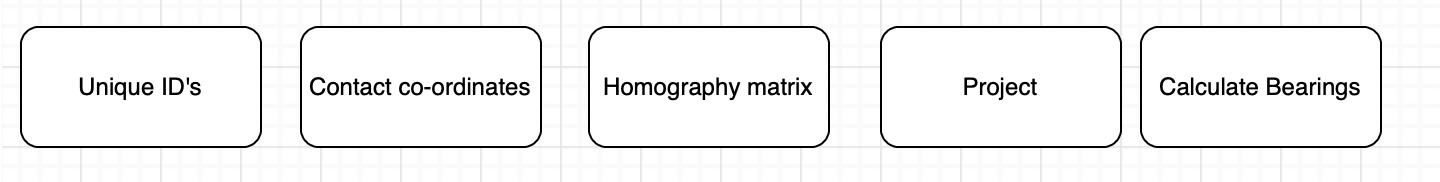
\includegraphics[width=1.0\columnwidth]{temp.png} 
\end{tabular}
\captionof{figure}{Data pipeline overview}
\label{pipeline}

\section{Data Collection}

The Dybbølsbro intersection in Copenhagen was chosen as the location for our primary data collection. 
The Dybbølsbro intersection faces several traffic flow challenges as a result development in the immediate vicinity as well as being a large intersection.
These challenges make the Dybbølsbro intersection one of the more extreme in Copenhagen and would serve as a good base to this quantitative analysis method. 
As Dybbølsbro is a large intersection we use two cameras on opposite side of the intersection in order to get a good overview of the intersection regardless of the traffic obstructing views.

\subsection{Recording Location}

There are three consideration to take into account when applying these methods to an intersection.
\begin{itemize}
	\item1. Intersection size.
	\item2. Camera mounting points.
	\item3. Intersection composition
\end{itemize}

\subsection{Camera Selection}

Modern mobile phones offer high resolution and quality cameras in a compact design. We used an LG G6 and a Samsung S7 Edge for recording the intersection.
These devices offer wide enough field-of-views (FOV) to record the parts of the intersection we are interested in from the selected mounting locations.
FOV being the maximum area a camera can image. A formal method of selecting a recording device would be to select one that has a large enough FOV that can image the entire intersection 
from the mounting position that is closes to the intersection. Given a recording location we can calculate the FOV needed using equation \ref{eq:1}.
If $\theta > FOV$ then the FOV is too small.
\begin{equation}
    \theta = tan^-1(\frac{\frac{width}{2}}{adjacent}) * 2\label{eq:1}
  \end{equation}

\ \\ 
  \begin{figure}[h]
    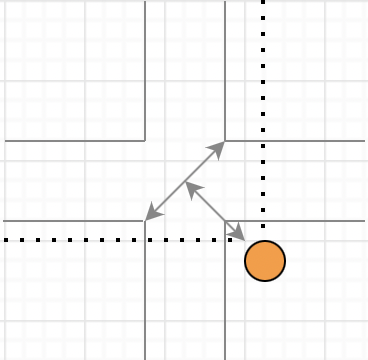
\includegraphics[scale=1.0]{location.png}
    \centering 
    \end{figure}
    \captionof{figure}{Barrel Distortion}
    \label{Camera location}

Battery life should also being considered depending on the amount of intended recording. 149MB per 1 min at 30FPS

\section{Data Processing}

\ \\ 
\noindent
\begin{tabular}{@{}cc}
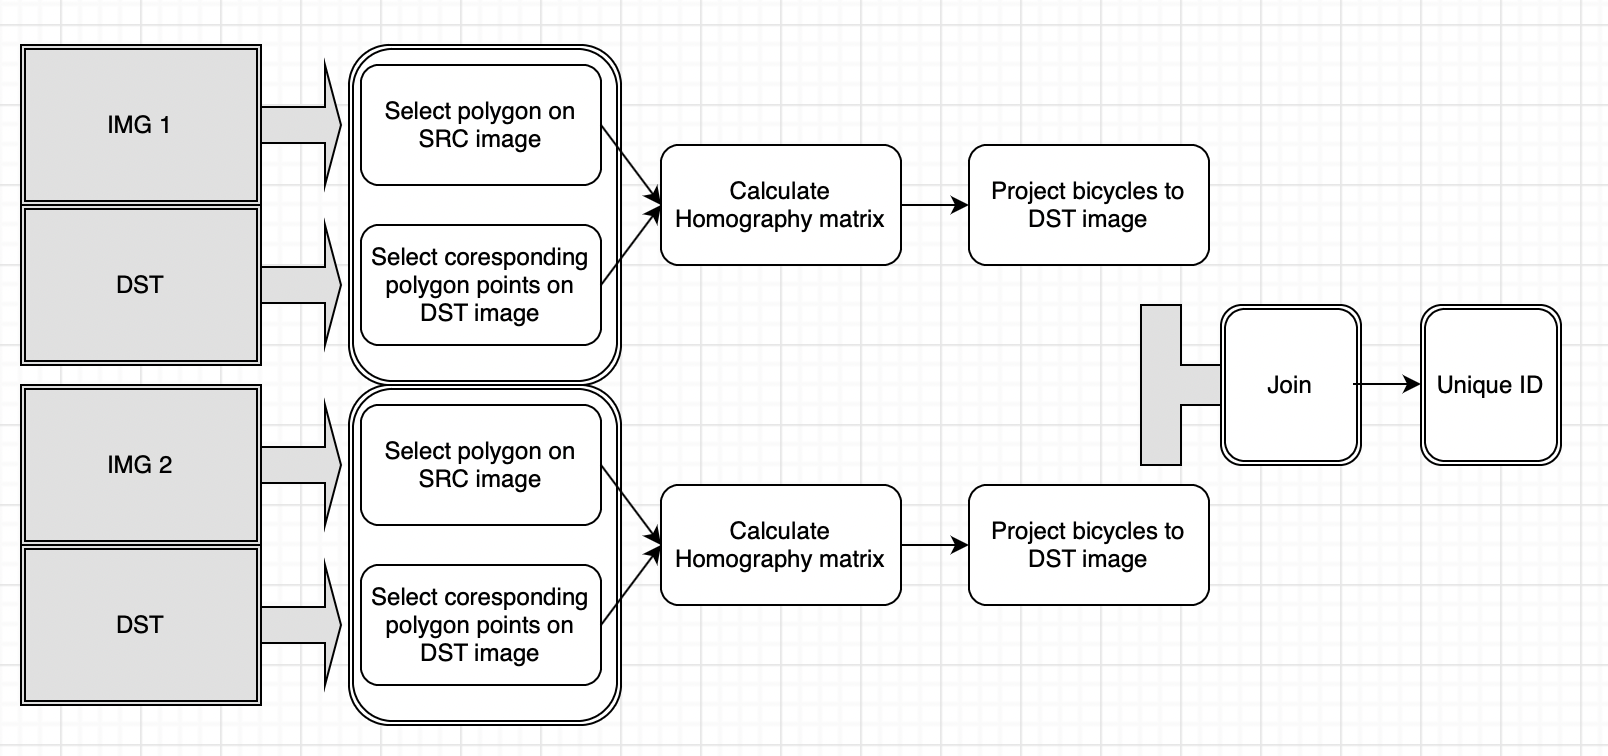
\includegraphics[width=1.0\columnwidth]{data_flow.png} 
\end{tabular}
\captionof{figure}{Data Pipeline}
\label{data}


Figure \ref{data} offers a general overview of the data processing steps. The processing happens on two 
video sources that are cut to the same time period. No special hardware is required, but a CUDA enabled GPU
device would speed up the object detection process.
\ \\
\subsection{Distortion Correction}

Wide angle camera lenses such as that on the LG G6 used in this study produce images that have an optical aberration where straight lines appear bent. 
The specific type being barrel distortion such as in figure \ref{distortion}, where lines curve inwards in a shape of a barrel.

\ \\ 
\begin{figure}[h]
  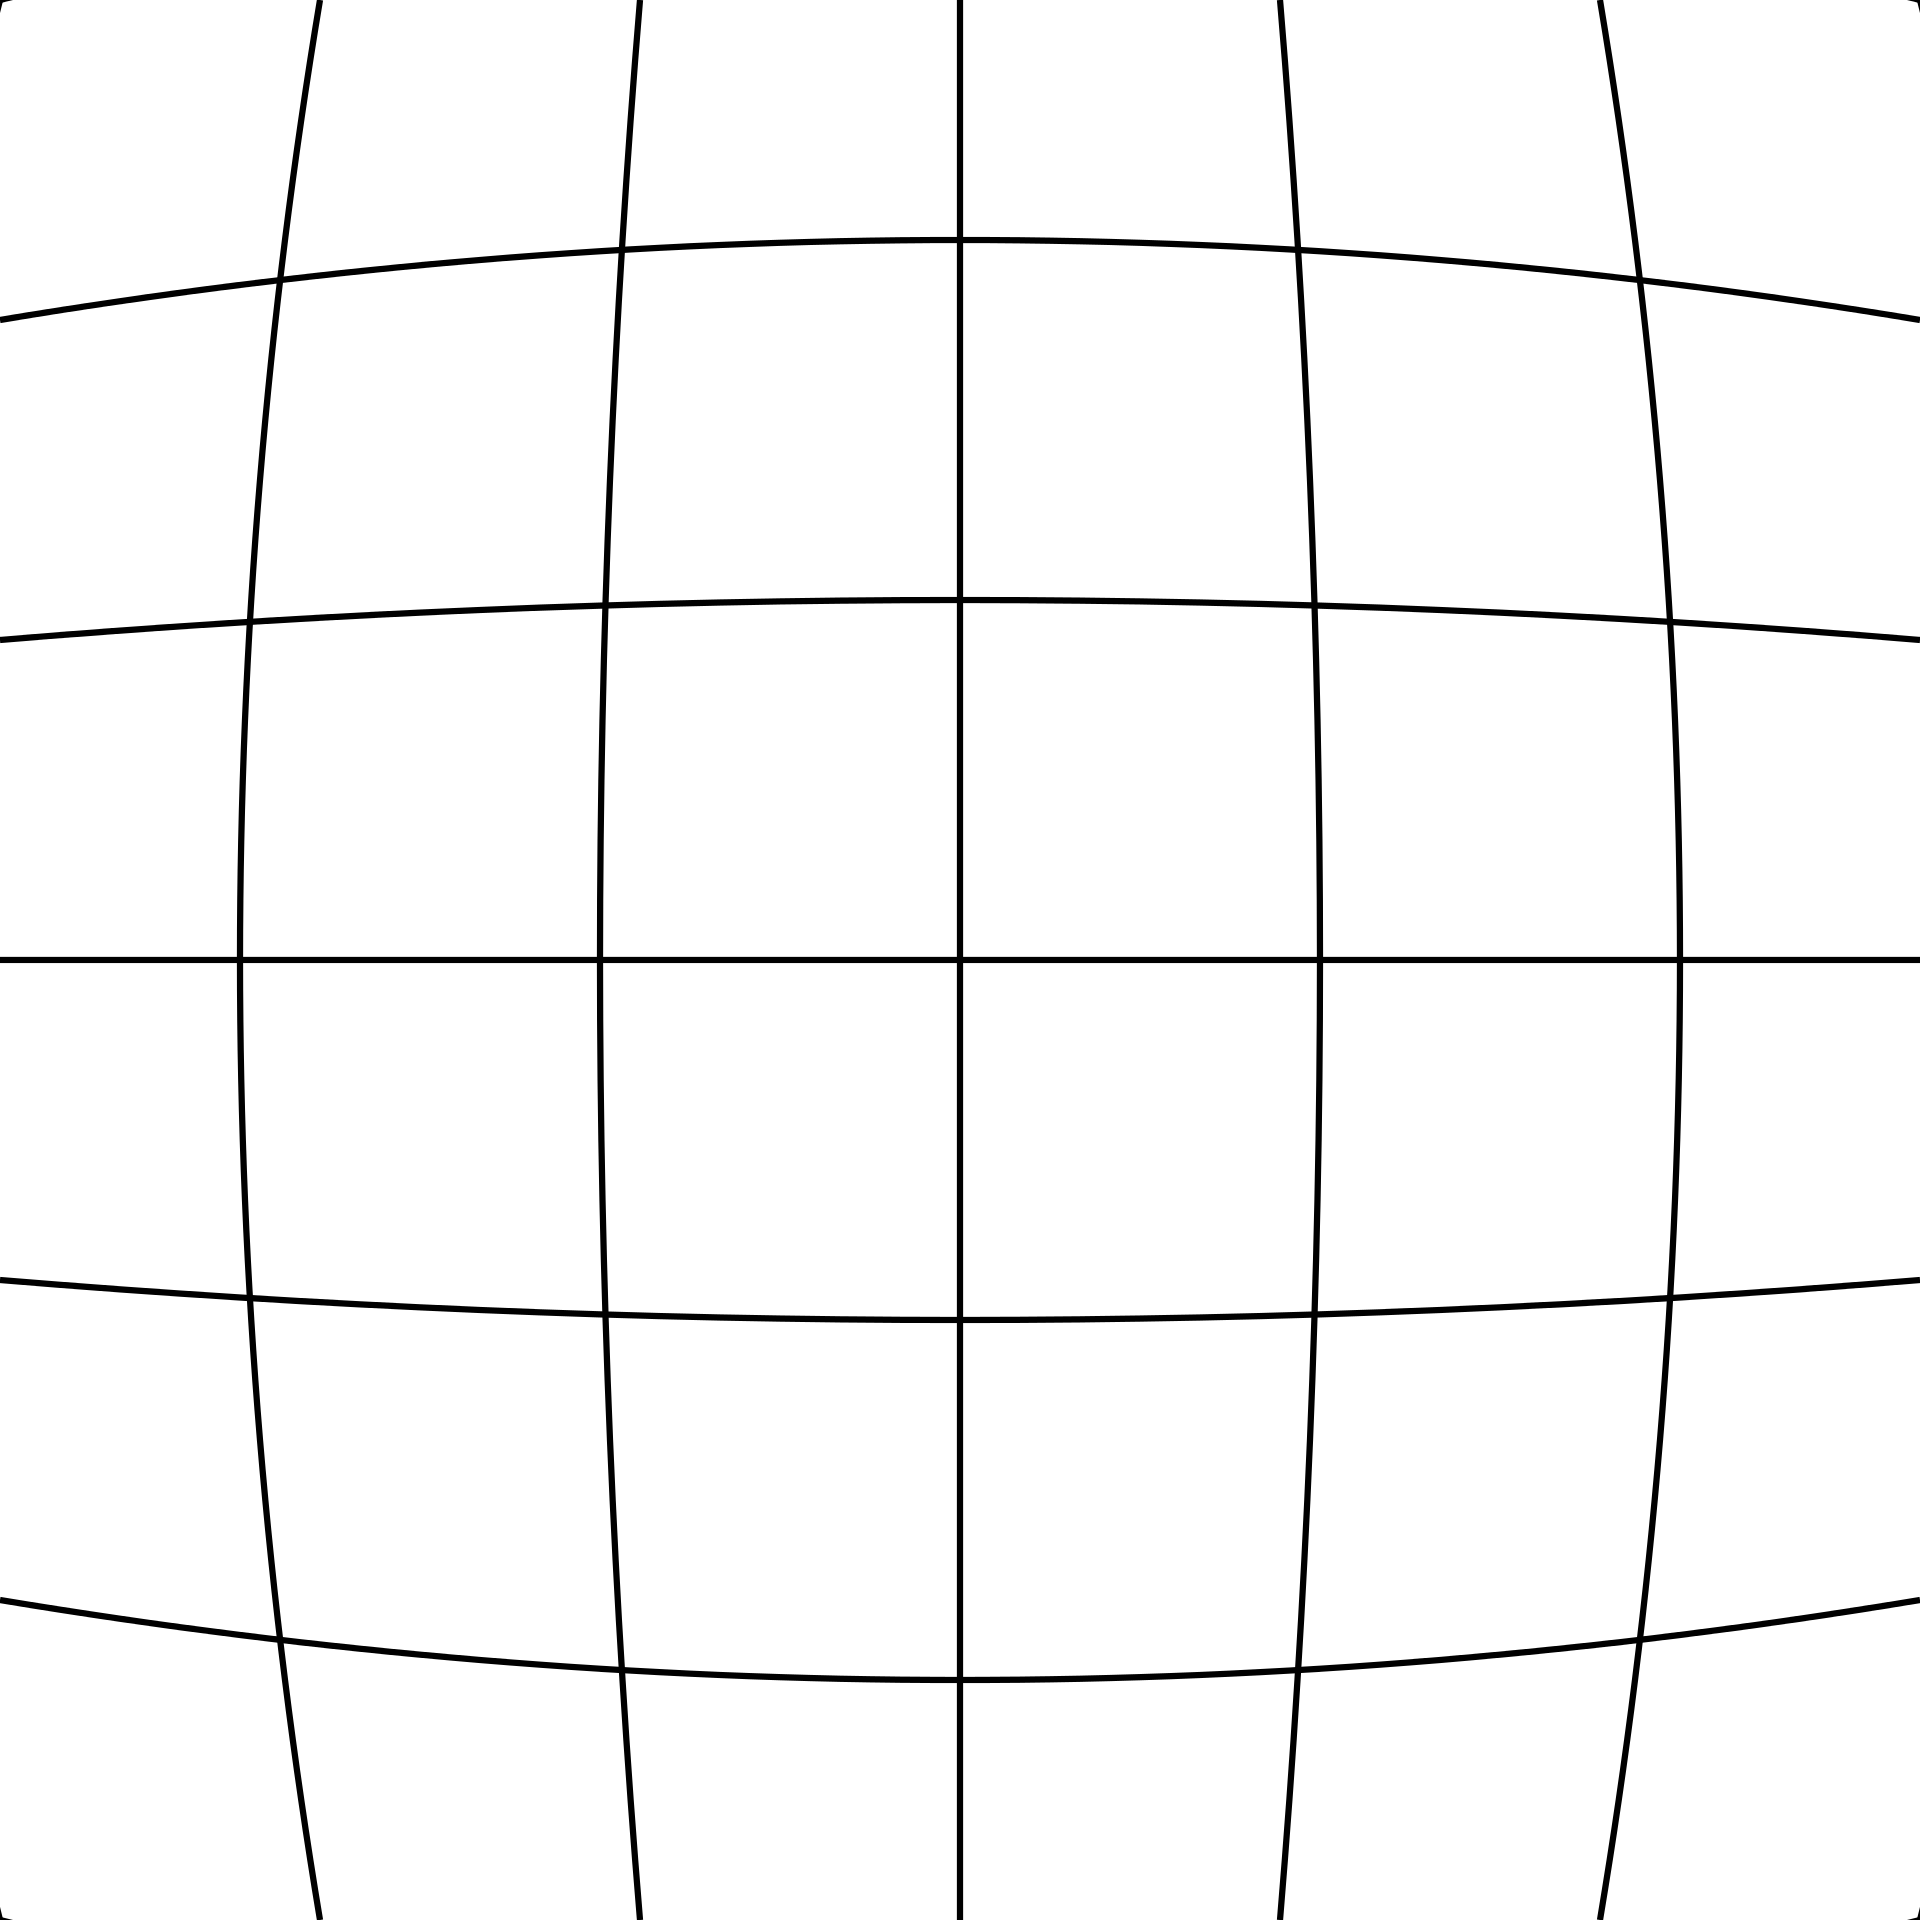
\includegraphics[scale=0.05]{Barrel_distortion.svg.png}
  \centering 
  \end{figure}
  \captionof{figure}{Barrel Distortion}
  \label{distortion}

\ \\
This can lead to incorrect projection and therefore joining of video sources later on.
To correct for this we make use of OpenCVs \cite{noauthor_opencv/opencv_2021} camera calibration toolbox.

Explain this a bit more. Formulas
\ \\
\subsection{Object Detection}

The raw video is output as a .mp4 file this video file is if fed to YOLO v5 for object detection. YOLO, You Only Look Once,
is a real-time object detection algorithm. ....Explain more.... 
\ \\ 
Why YOLO v5?
\ \\ 
Objects are detected each frame and represented as bounding boxes.
The output from YOLO is as follows: \[ [frame id][xmin][ymin][xmax][ymax][confidence]  \]

The min and max values for x and y represent a bounding box for the identified bicylce.

Figure \ref{data_pipeline} demonstrates the data pipeline that the output from YOLO is fed through. .
\ \\
\subsection{Homography Matrix}

First explain the concept of the homography matrix.
\ \\ 
\begin{figure}[h]
  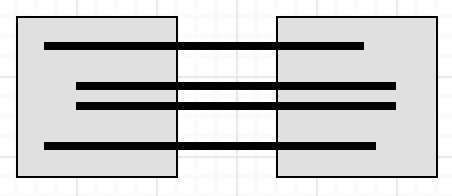
\includegraphics[scale=1.0]{Homography_proj.png}
  \centering 
  \end{figure}
  \captionof{figure}{SR to DST}
  \label{homography}

To transform the data to onto the a new plane view we needed to find the homography matrix, which is a transformation matrix between two planes \cite{hartley_zisserman_2004}.
The homography matrix (H) is a 3×3 matrix with 8 degrees of freedom, this allows the transformation of the cycling objects $P(x_r, y_r)$ to a 
top-down aerial view $P(x_i, y_i)$. The top-down view being an aerial image of the Dybbelobrø intersection and P being the image coordinates in pixel units.

\begin{equation}
  P = HQ\label{eq:2}
\end{equation} 

\begin{align}
\label{eq:3}
  \begin{bmatrix}
    x_{i} \\
    y_{i} \\
    z_{i} \\
  \end{bmatrix}
  &= \begin{bmatrix}
      h_1 & h_2 & h_3 \\
      h_4 & h_5 & h_6 \\
      h_7 & h_8 & h_9 \\
  \end{bmatrix}
  \begin{bmatrix}
    x_{r} \\
    y_{r} \\
    z_{r} \\
  \end{bmatrix}
\end{align}
\subsection{Projection}

After finding the homography matrix we can now project to contact points of the bicycle and the road surface onto the destination
image being an aerial view of Dybbelsbrø. This is achieved by applying $z$ to each point as a constant so as to create $Q(x_i, y_i, 1)$ and then we multipy it by 
homography matrix. 
\ \\
\subsection{Merging Sources}

To merge the data from the two video sources we take a naive approach. As the cameras are setup on
opposite siders of the intersection for optimal coverage we simply cut the video sources in half along the halfway point between
the two cameras along the intersection. The data is then merged.
\ \\
\subsection{Multiple object tracking}

In order to connect observations into trajectories of individual cyclist we apply 
simple online and real time tracking algorithm, SORT \cite{abewley_abewley/sort_2021}, as initially described in \cite{Bewley2016_sort}. 
SORT aims to address the problem of multiple object tracking (MOT) where object across frames needs to be connected. 
Explain more about SORT predict bbox then iou for actualy bbox.

The algorithm returns the bounding boxes along with a unique ID associated with each observation.

Using the bounding boxes we calculate the (x, y) co-ordinates of the observation and shift the y value down onto 
the same plane as the street so as to have the conact point of a bicycles and the street.

\section{Data Exploration}

There are two objectives for the data exploration.
\begin{itemize}
	\item1. Rainbow Tracks - Desire path discovery
	\item2. Alert Zones - For behaviour observations and counts
\end{itemize}

\subsection{Rainbow Tracks}

\ \\ 
\noindent
\begin{tabular}{@{}cc}
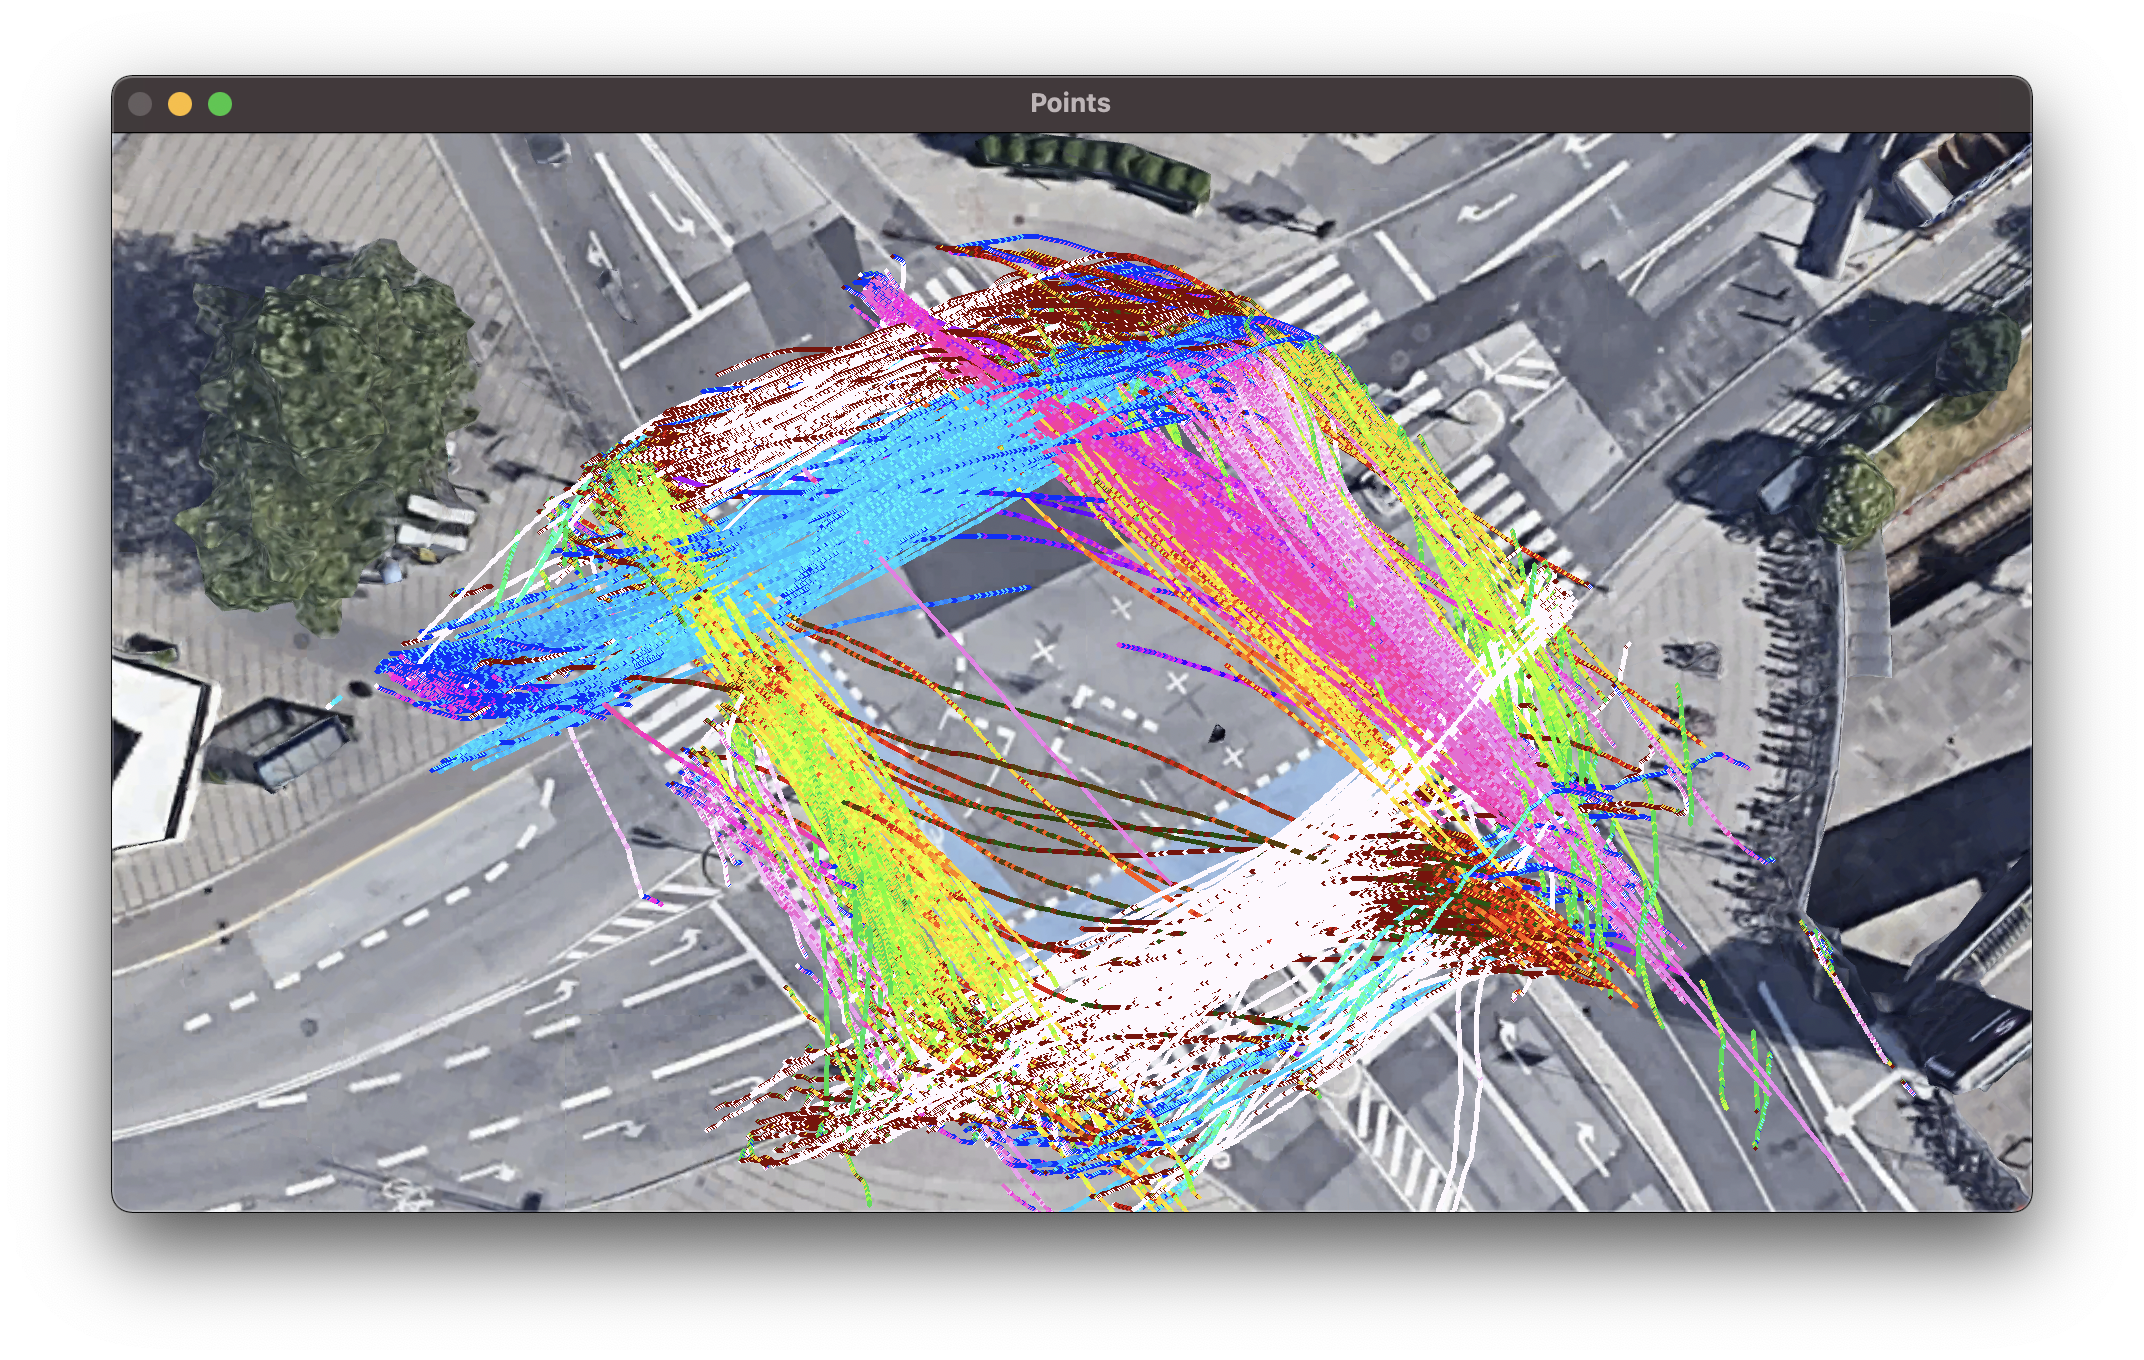
\includegraphics[width=1.0\columnwidth]{rainbow.png} 
\end{tabular}
\captionof{figure}{Rainbow}
\label{Rainbow}

To find aggregated desire lines from the data we took an approach which we call "Rainbow tracks". This involves coloring tracks by the bearing between consequtive points in each 
trajectory, after calculating the bearing we then get a color from a gardient color wheel. This approach has the added benefit of encoding direction into 
each track.
Maybe just an equation demonstaring the bearing calculation.
\ \\ 
\begin{equation}
  UniqueID_i = [(x_1, y_1)...(x_a+1, y_a+1)]\label{eq:3}
\end{equation}

\subsection{Alert Zones and Counts}

We created a "Tool name", that allows the defining of certain areas as "Red zones". These zones are provide us with easy reference to activty in the zones throught the videos.
Using these zones we can count cyclist and observe their behaviour at points on the intersection that might be difficult or
problematic.

Picture of interface?

% As a baseline we deploy a vanilla OpenDataCam setup using its built-in tools for object counting and path recording.
% From the OpenDataCam GUI it's possible to visually inspect the detected objects and draw line counters 
% which keep track of the total number of objects passing the line given a certain areal threshold and approach angle. 
% The line counters are bi-directional and segment totals based on the mode of transportation.

% \ \\
% The baseline will focus on the capabilities of only applying OpenDataCam and its tools. This will mostly be "trafic shares" for 
% different paths and directions. 
% \\ 
% We then go on with further data processing as an extension. The main goal is to have a tool catered to analyzing cyclists, capturing
% discrete desire lines (with magnitude) and the ability to "hook into" video material for certain scenarios.

% \subsection{Hardware}
% The pipeline for our setup is shown below on figure \ref{system}. OpenDataCam uses the Yolo4 weights to localize cyclists and pedestrians.
% Processing was executed on an ARM based NVIDIA Jetson Xavier NX (development board) equipped with a 384-core NVIDIA Volta GPU
% and 8GB of memmory. 

% \raggedbottom
% \noindent
% \begin{tabular}{@{}cc}
% 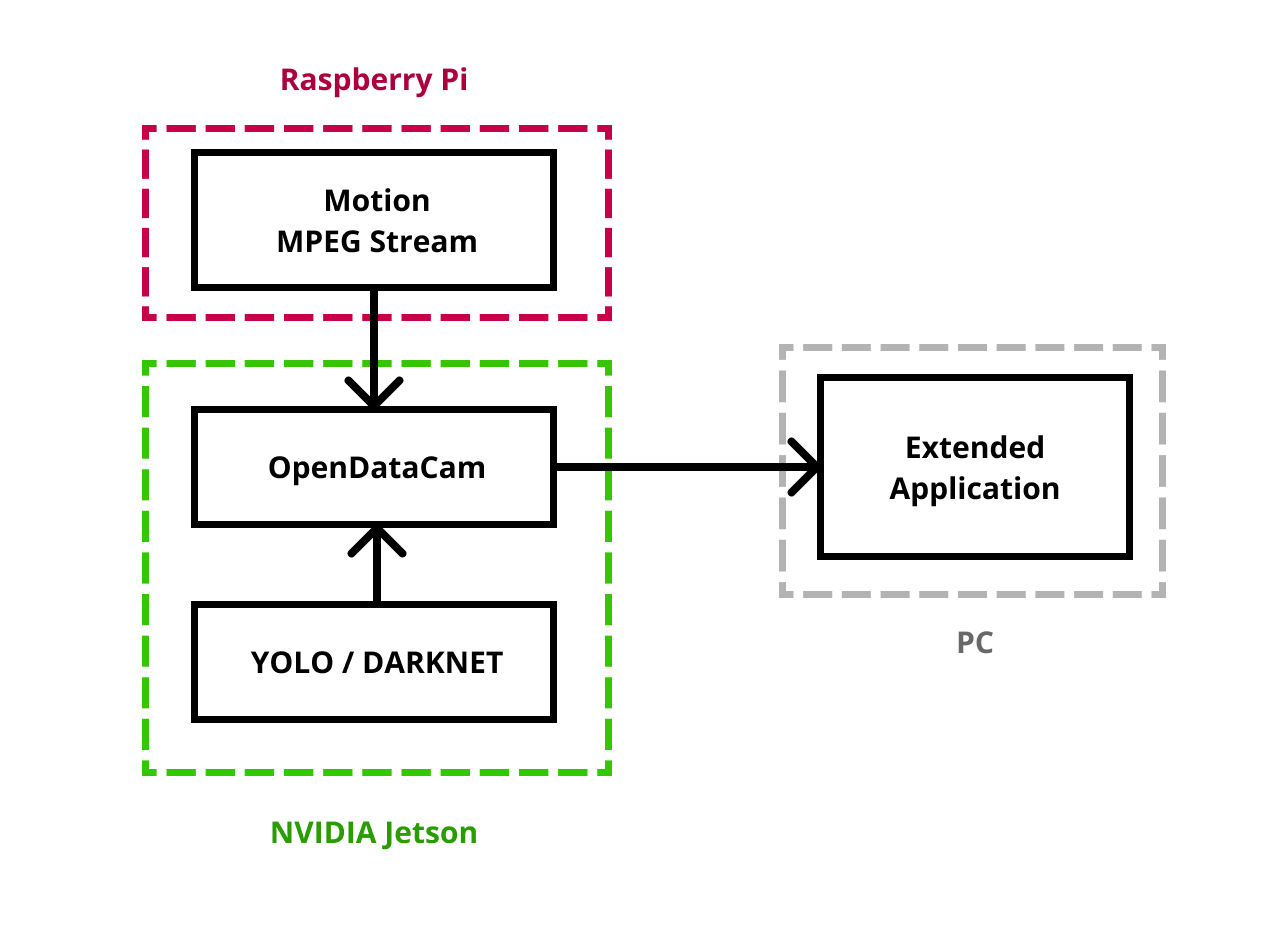
\includegraphics[width=1.0\columnwidth]{system} 
% \end{tabular}
% \captionof{figure}{System overview}
% \label{system}

% \ \\
% The video feed for YOLO is provided through the OpenDataCam interface, which allows for real-time analysis through an onboard camera
% or a video stream from an IP camera. 

% \ \\
% For further analysis the raw data from the recordings was exported in the form of CSV and JSON files. This includes both the low-level
% object detection (bounding-boxes, frame reference, confidence levels etc.) and the totals from the line counters.

% \subsection{Trajectory projection}
% The video footage was analyzed using OpenDataCam which is an abstraction layer on top of Yolo. Yolo being an object detection library for object detection in images.
% Once the video is analyzed by OpenDataCam, we receive a .json file containing a Unique ID for each identified cyclist that is detected for each frame of the video file. 
% The unique ID is accompanied by bounding box coordinates of the detected bicycle on the frame. 
% The center-bottom coordinates of the bounding box over multiple frames represents the track of an identified bicycle.

% \ \\
% By assuming the road as a 2D plane, hereby ignoring any non-linear deformations (e.g. from lens distortion or curvature of the pavement), 
% we can transform the pixel positions from the video to real-world 2D coordinates. 
% We calculate the \textit{homography matrix}, describing the transformation from one plane to another, by mapping four reference points from each frame (figure \ref{projection_figure}).

% \raggedbottom
% \ \\ 
% \noindent
% \begin{tabular}{@{}cc}
% 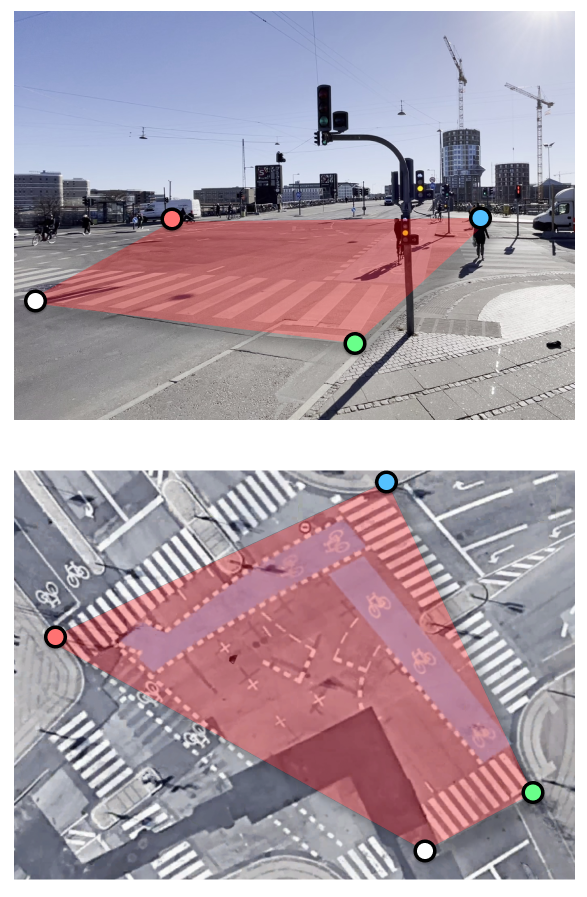
\includegraphics[width=1.0\columnwidth]{projection_figure} 
% \end{tabular}
% \captionof{figure}{Reference points on map projection}
% \label{projection_figure}



% \subsection{Trajectory clustering}
% Desire Lines

% \subsection{Catching unexpected behavior}
% "Red zones" defined by a certain area, speed og trajectory can provide context (through video) when activated. 
% % features, model, evaluation

\chapter{Results and Discussion}

% Results and Discussion could also be two separate chapters

\chapter{Conclusion}
\label{conclusion}

conclude and restate main finding, answer research question

point to limitations and future work
%\section{Limitations}
%As our study was limited in the time and resources available, it is far from conclusive. We will describe a few of its limitations below.




%----------------------------------------------------------------------------------------
%	BIBLIOGRAPHY
%----------------------------------------------------------------------------------------

\bibliographystyle{chicago} 
\bibliography{thesisbiblio}


%----------------------------------------------------------------------------------------
%	APPENDICES
%----------------------------------------------------------------------------------------
\newpage
\appendix
\chapter{Appendix}



\end{document}



